\documentclass{article}
\usepackage[margin=0.5in]{geometry}
\usepackage{graphicx}
\usepackage{wrapfig}
\usepackage{amsmath}
\graphicspath{{Images/}}
\usepackage[ampersand]{easylist}
\usepackage{url}


\usepackage{natbib}
\bibliographystyle{abbrvnat}
\setcitestyle{authoryear,open={(},close={)}}

\begin{document}
	
\title{Single Camera Autonomous Vehicle Navigation Localisation Implementation Discussion}
\author{Michael McDonnell}
\date{}
\maketitle

\section{Overview}
During the course of development of the single camera autonomous vehicle navigation localisation system, several implementation points were identified which were deemed outside the scope of discussion in the original article however are included here in an effort to preserve the information. This information is of particular importance to those interested in implementing or extending the system.


\section{System parameters.} The system has a range of parameters to be specified which allow customisation to both vehicle and route specifications. System parameters include: 

\begin{easylist}
	& \textbf{Camera parameters.} 
	&& \textbf{Field of view.} The camera field of view affects the visibility of road surfaces off the direct line of travel at the close edges of the vehicle, especially after IPM is applied. If the field of view is too narrow, route features such as side streets may be lost prematurely. As such, a field of view with reasonable vision to the left and right of the driving surface in the near distance is required.	
	&& \textbf{Frame resolution.} This system remains effective at lower resolutions so the full resolution of the camera frame may not be required. While larger frames contain more detail in general the system can trade some resolution for computational time savings without significant losses. Frame resolutions used in testing varied from 512px to 150px widths. 
	&& \textbf{Frame processing frequency.} While not strictly a camera parameter, the frequency with which the system processes the frames is a key consideration and will generally relate to the processing speed of the implementation. A lower frequency of frame processing results in a higher likelihood of route feature tracking errors and less redundancy in any detection failures. Frame frequency for this test was as low as 10Hz with no noticeable degradation in feature detection or optical flow tracking. This parameter should be considered in context with resolution to ensure that optical flow tracking remains effective.
	& \textbf{Road surface detection.}
	&& \textbf{Assumed road surface region.} The histogram backprojection relies on a specified area in front of the vehicle to be sampled for the histogram for backprojection. This region will vary based on the physical setup of the vehicle and camera mount and should be chosen carefully to avoid introduction of additional noise such as road edges. The size of this region is dependant on the camera field of view; a narrow camera field of view will restrict the area that can be reliably sampled as road surface.
	&& \textbf{Feature detection probability threshold.} This value is considered when determining if a feature has been detected. A value of 1.0 will require each pixel of the feature mask to be over a road surface pixel with a probability of 1.0. The only occasion this is feasible is in the case the detected road surface is a purely binary thresholded mask. Realistically the detection threshold probability needs to be less than 1.0 to account for noise and uncertainty in the detected road surface.
	& \textbf{Feature development}
	&& \textbf{Image pixel to real world distance ratio.} This can be determined from the IPM procedure based on known real world distances as projected after IPM occurs. This is required for the development of route feature masks at an accurate scale. 
	&& \textbf{Route feature mask width.} The pixel width to use when developing the route feature mask. This width does not need to represent a full vehicle width as the driving line mask will ensure the vehicle can pass through the feature. In the development of this system, the route feature mask width was 25\% of the vehicle width. If this width is too great there is a risk that the combined driving line and feature mask may be wider than the feature itself, leading to a failure to detect the feature.
	&& \textbf{Driving line mask width.} Related to above however this needs to have a real world width to comfortably accommodate the vehicle width to ensure driving line through the feature will ensure the vehicle remains on the detected road surface.
\end{easylist}

These parameters directly impact the effectiveness of the system however are generally easy to tune as the entire system is human interpretable thus the effect of a parameter can be directly observed and understood.


\section{Road surface centreline detection}

While vehicle position and orientation on the road is a critical input to a controller, it was not explicitly covered as part of this system. A general approach slightly modified from that outlined by \citet{canneyAndHoughLanes} to suit this system is to identify the central point on a road surface is to apply edge detection to the detected road surface pixels followed by identifying straight line candidates using the Hough transform. The basic approach would be as follows: 

\begin{easylist}
	& Identify local window of interest in the near ground to vehicle.
	& Use edge detection such as the Canny algorithm to identify road edge pixels inside window of interest.
	& Identify candidate lines using Hough Transform.
	& Select strongest candidate lines for left and right portions of the window, corresponding to the estimated left and right road edge lines.
	& Identify road centreline as midline between left and right detected edge lines.
	& Determine desired steering direction based on detected centreline pixel offset from vehicle centreline \footnote{The vehicle centreline will correspond to the image centre assuming the camera is position centrally. If the vehicle mounted camera is offset, this `centre pixel line' will need to be manually identified and stored prior to operation.}
\end{easylist}

This approach can be applied to either the camera perspective image or the IPM transformed image. In the former case the perspective effect where the left road edge line will be angled to the right and vice versa for right edges, tending to the vanishing point, allows easy segregation of left and right road surface lines. By contrast the IPM transformed road edges will be parallel thus rely on positional information only to separate the left and right road surface lines. Alternatively more advanced methods such as the Support Vector Machine approach suggested by \citet{moncularLaneDetectAndTrack} may be more robust and may additionally inform the road surface detection.



\textbf{Extension of feature masks.} As designed, the current system only considers the main feature node and immediate connections. As the feature node is placed centrally, the approach node distance results in only masking a small portion of the full image. An improvement is to extend the sub masks from the feature node to the full extent of the mask image size. This would involve each sub mask drawing additional relevant node connections until the relative position takes the line off the edge of the image. The resulting mask will be a full representation of the approach route to the feature.

\begin{wrapfigure}[20]{r}{0.35\textwidth} %this figure will be at the right
	\centering
	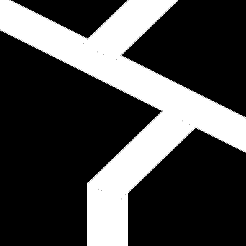
\includegraphics[width=0.35\textwidth]{complexFeatureApproach.png}
	\caption{An example of a complex approach to a feature which may undermine the current system feature detection.}
	\label{f:complexFeatureApproach}
\end{wrapfigure}

\section{Rotation of feature masks.} The current implementation has the system generating feature masks of the route feature as it will be approached and assumes a linear approach. This is a reasonable assumption for close in detection however it may fall down if complex approaches to route features are encountered. A more robust solution would involve developing the extended feature mask as outlined above and aligning the mask to the approach direction at the frame the feature will be detected. This would entail developing the mask and once developed, the mask can then be rotated so the approach line is vertical at the base of the image. On arrival at a feature node on the approach, the mask will be regenerated and reoriented. This approach takes advantage of the fact that the route between two nodes can be assumed as linear and will ensure the feature mask orientation will match the detected road more closely. 

An example of a complex approach to a feature is included as Fig. \ref{f:complexFeatureApproach}. In this instance as the vehicle encounters the first bend, the feature model mask will no longer have the correct orientation and result in a loss of feature tracking. 


\section{Navigation extension options.} While it was not explicitly considered as a feature, any road feature with a sharp enough angle between points can be used as a feature. This is particularly helpful if an aim is to identify a `true' position outside GPS error as bends in a road can be used as additional features without requiring additional intersecting roads. Additionally while this system was designed with a supporting GPS in mind to estimate anticipated feature arrival, as developed it does not rely on positional information specifically. Indeed assuming that relevant route feature data is stored, this system can work `offline' using the features as directions in a similar way a human navigator may. Integrating the output of this system with other sensors such as GPS offers additional localisation benefits. \citet{probabalisticRobotics} discuss Markov and extended Kalman filter localisation techniques that may be applicable to this system and have the potential to result in improved positional estimation.

\section{IPM maximum distance}\label{s:ipmMaxDist}

Initial implementations of the system used IPM transformations which aimed to maximise the visible `top down' road surface by choosing points close to the horizon in the perspective image to transform which corresponded to distances of approximately 100m. While this approach is effective where there are long stretches of visible road it has significant failure points. If the relative distances are maintained it results in a narrowing of the road surface in the top down view. Additionally it generates significantly more interpolated data (`stretched pixels') and results in a small portion of detected road surface where the road is not straight which is particularly evident when approaching a corner. 

Distances in the order of 15-20m were determined to be the most effective for road surface detection in this implementation. This results in less interpolation of data and a reasonable road surface coverage even when approaching corners. The downside to this approach is it is only `looking ahead' a shorter range so any controller that is implemented will likely need to anticipate approaching features to manage velocity changes. 

\section{Opportunities for future work} \label{s:improvements}

\subsection{Estimation of road surface in IPM voids}

In the current implementation, the `void' in the IPM transformed image (where no information is contained) is not considered. There is scope for road surface estimation in this area based off preceding frames. As detected road surface moves outside the IPM transformed image, there is scope for future work to interpolate the estimated position of road surface from prior `in frame' detection.

\subsection{Feature bracketing in lieu of optical flow estimation}

It was determined the optical flow estimation added in the order of 60ms processing time per frame. This allowed effective feature tracking in testing however a heuristic for an intelligent `bracketing' update procedure may result in computational savings as the 60ms addition from optical flow represents 5-6 feature mask operations.

While this may be an avenue of interest, by itself it does result in a non-smooth positional tracking as the feature location will `jump around' based on bracketing steps. This may be addressed further through Kalman filtering in a more advanced implementation.

\subsection{Integration with Fuzzy Logic.} \citet{fuzzySail} present results demonstrating a very effective combination fuzzy control system for a sailing boat including the ability to tack and jibe. \citet{fuzzyGrove} outlined significant improvements in using fuzzy logic for sensor fusion and control of autonomous vehicles operating in citrus grove alleys. The system discussed in this paper involves probability based decisions throughout the process and may be a good candidate for integration with Fuzzy logic decision making and/or control.

\subsection{Known road map histograms.} The histogram backprojection uses an average histogram over the previous 5 frames. This is effective for slowly changing road surfaces however can lead to brief road surface loss when moving from one surface to another. An alternate option is to have a bank of representative road surfaces, including areas under specific lighting conditions, to use for the backprojection and consider the maximum probability over the range of surfaces as each pixel's probability of being a road surface. This can also be combined with the rolling average to provide a more robust assessment as well as categorise road surfaces. 

\subsection{Optimisation of system parameters}
There are a large range of system parameters that need to be manually tuned for implementation including selection of IPM transformation points as outlined in Section \ref{s:ipmMaxDist}, regions of interest for histogram backprojection and optical flow and processing frequency and resolution. While some of these parameters are difficult to automate, parameters such as image frame resolution and optical flow window bounds may be suitable for multi objective optimisation automation, especially when considering the tradeoff between resolution accuracy and individual frame computational processing time.

\newpage
\bibliography{References}

\end{document}